\documentclass[12pt]{article}

\usepackage{tikz}

\title{Matematica}
\author{Simone Balducci}
\date{}

\begin{document}
\maketitle
\section{Probabilita' e statistica}
\subsection{Probabilita'}
Si consideri una certa operazione, quale l'estrazione di una carta da un mazzo o il lancio di un dato. Ci sono tanti possibili risultati per queste operazioni. L'insieme di tutti i risultati possibili forma lo \textit{spazio campionario} $\Omega$, mentre uno di questi possibili risultati prende il nome di evento, e rappresenta quindi un sottoinsieme dello spazio campionario. \\
La probabilita' associata a un evento e' data da
$$
	p(E) = \frac{|E|}{|\Omega|}
$$
dove $|E|$ indica il numero di casi possibili che rientrano nella descrizione dell'evento e $|\Omega|$ sono tutti i casi possibili. \\
Ad esempio, nel caso dell'estrazione della carta da un mazzo di 52 carte, l'evento "Esce una carta con il numero 4" e' verificato in 4 casi dei 52 possibili (un caso per ogni seme). Ne risulta che questo evento ha probabilita' 
$$
	p(E) = \frac{4}{52} = 1/13 
$$
\subsubsection{Probabilita' condizionata e dipendenza}
Il concetto di probabilita' condizionata e' di fondamentale importanza per la sua utilita' pratica e perche' permette di introdurre in maniera intuitiva il concetto di eventi indipendenti. \\
Si definisce la probabilita' condizionata dell'evento $A$ noto l'evento $B$ come:
$$
	p(A|B) = \frac{A \cap B}{B}
$$
Il significato di questa probabilita' e' quello di indicare la probabilita' che un evento, l'evento $A$, avvenga sapendo che l'evento $B$ e' avvenuto. In sostanza, calcolando questa probabilita' noi supponiamo di avere un'informazione in piu', e spesso questa modifica la probabilita' a priori che $A$ avvenga. \\ \\
Un esempio molto semplice di questo concetto e' il seguente: \\
Supponiamo di avere un classico mazzo di carte da 52. L'evento $A$ e' l'evento "viene pescato il 2 di cuori", mentre l'evento $B$ e' "viene pescata una carta di cuori" e consideriamo anche l'evento $C$, che dice "viene pescata una carta di picche". \\
A questo punto possiamo calcolare le probabilita' condizionate. \\
Il fatto che gli eventi $B$ o $C$ avvengano, va a cambiare la probabilita' che $A$ avvenga. Infatti, la probabilita' che $A$ avvenga, a priori, e' $1/52$. Tuttavia, se sappiamo che $B$ si e' verificato, la probabilita' di pescare il 2 di cuori diventa molto piu' alta, ovvero
$$
	p(A|B) = \frac{1}{13}
$$
questo perche' sapere che e' stata una pescata una carta di cuori, va a diminuire il numero di carte che e' possibile pescare. \\
Similmente, se consideriamo verificato l'evento $C$, abbiamo di nuovo che la probabilita' che $A$ si verifichi cambia. In particolare tale probabilita' diventa nulla, perche' non si puo' pescare il 2 di cuori se si pesca una carta di picche, quindi
$$
	p(A|B) = 0
$$

Si puo' ora introdurre il fondamentale concetto di eventi indipendenti. \\
Intuitivamente, due eventi sono indipendenti se il fatto che uno avvenga o no non va a modificare la probabilita' che l'altro avvenga. \\
Matematicamente, si dice che la probabilita' condizionata dell'evento e' uguale alla probabilita' a priori:
$$	
	p(A|B) = p(A)
$$
Un primo esempio molto semplice e' il seguente: Sapendo che Simone Balducci ha gli occhi verdi (evento B), qual e' la probabilita' che oggi piova (evento A)? Chiaramente l'evento B non influenza in alcun modo l'evento A. \\
Un altro esempio, che a volte puo' risultare fuorviante, riguarda il lancio di una moneta. Supponiamo di lanciare una moneta 2 volte: Sapendo che nel primo lancio esce testa, qual e' la probabilita' che esca testa anche al secondo lancio? Questa probabilita' e' sempre $1/2$, quindi i due eventi sono indipendenti. Intuitivamente, e' chiaro che il risultato del lancio di una moneta non dipende dai risultati precendenti. Qualcuno potrebbe essere fuorviato dal fatto che ottenere lo stesso risultato (ad esempio testa) a ogni lancio e' qualcosa di improbabile, dopo un certo numero di lanci. Questo e' vero, ma in questo caso si parla di probabilita' dell'intersezione di eventi, non della probabilita' del singolo evento. \\ \\
Se due eventi sono indipendenti, la probabilita' dell'intersezione (ovvero la probabilita' che avengano entrambi contemporaneamente) e' data semplicemente dal prodotto dei due
$$
	p(A \cap B) = p(A)p(B)
$$
Quindi, tornando al caso del lancio di una moneta, se lanciamo la moneta due volte e ci chiediamo la probabilita' che esca testa due volte di fila, questa e' data semplicemente dal prodotto delle due probabilita', quindi $1/4$. \\ \\
Per l'esempio precedente, dei lanci di moneta successivi, si puo' usare uno strumento molto potente, che e' quello dei diagrammi ad albero.
\begin{center}
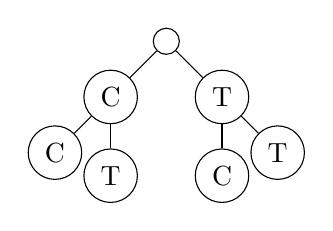
\begin{tikzpicture}[main/.style = {draw,circle}]
\node[main] (1) {};
\node[main] (2) [below right of=1] {T};
\node[main] (3) [below left of=1] {C};
\node[main] (4) [below right of=2] {T};
\node[main] (5) [below of=2] {C};
\node[main] (6) [below of=3] {T};
\node[main] (7) [below left of=3] {C};
\draw (1) -- (2);
\draw (1) -- (3);
\draw (2) -- (4);
\draw (2) -- (5);
\draw (3) -- (6);
\draw (3) -- (7);
\end{tikzpicture}
\end{center}
Questo grafo e' formato da 4 rami, e ogni ramo rappresenta un possibile esito dei due lanci di moneta. Per quanto detto in precedenza, ognuno dei 4 rami e' equiprobabile, quindi la probabilita' di ognuno di essi e' $1/4$.
\subsubsection{Probabilita' dell'unione}
La probabilita' dell'unione di due eventi puo' essere compresa semplicemente immaginando gli insiemi. Immaginiamo due insiemi come due ovali su un piano, $A$ e $B$. La probabilita' dell'unione dei due eventi rappresenta la probabilita' che avvenga uno dei due, quindi intuitivamente le probabilita' vanno sommate. \\
Infatti, se consideriamo l'estrazione di una carta, se l'evento A e' "esce una carta cuori" e l'evento B e' "esce una carta quadri", se consideriamo l'unione dei due eventi vuol dire che siamo contento sia che esca una carta cuori che una quadri, quindi siamo passati da un quarto delle carte del mazzo a meta', raddoppiando la probabilita'
$$
	p(A\cup B) = p(A) + p(B) = \frac{13}{52} + \frac{13}{52} = \frac{26}{52} = \frac{1}{2}
$$
Tuttavia, il discorso non finisce qui. Infatti, immaginiamo che i due non siano disgiunti, e quindi che tra i due ci sia dell'overlap. In questo caso, sommando i due eventi staremmo considerando la zona in comune due volte. Per questo motivo, bisogna rimuovere la probabilita' dell'intersezione dei due eventi. E questo ci da' la formula finale e completa:
$$
	p(A\cup B) = p(A) + p(B) - p(A \cap B)
$$
Facciamo un esempio. \\
Consideriamo il lancio di un dado. Prendiamo come evento $A$ l'evento "esce un numero pari" e come evento $B$ "esce un numero maggiore o uguale a 3". I due eventi quindi si possono scrivere come
$$
	A = \{2,4,6\}
$$
$$
	B = \{3,4,5,6\}
$$
Si vede che ci sono dei numeri la cui uscita soddisferebbe entrambi gli eventi, ovvero si ha intersezione tra i due eventi. In particolare l'evento intersezione e' 
$$
	A\cap B = \{4,6\}
$$
Quindi, la probabilita' che avvenga $A$ oppure $B$ e'
$$
	p(A\cap B) = \frac{3}{6} + \frac{4}{6} - \frac{2}{6} = \frac{5}{6}
$$
e questo valore non deve soprendere, perche' vediamo chiaramente che con qualunque valore, a parte 1, si ha che uno dei due eventi e' soddisfatto. \\
E' importante stressare un'ultima volta l'importanza di togliere la probabilita' dell'intersezione, perche' e' molto comune dimenticare quel termine. \\
Se noi sommassimo semplicemente le probabilita' dei due eventi, sarebbe come dire "ok quindi vincero' questo gioco se uscira' 2, 3, 4, 5, 6, 4 o 6, quindi ci sono 7 casi possibili che mi farebbero vincere". Ma questo chiaramente non ha senso, perche' due di quei casi sono stati contati due volte. Addirittura, se non togliessimo l'intersezione, la probabilita' dell'unione verrebbe maggiore di 1, che e' chiaramente impossibile.
\subsubsection{Teorema di Bayes}
Il teorema di Bayes riguarda la probabilita' condizionata e risponde a una domanda. Se io so una probabilita' condizionata, come trovo l'inversa? Ovvero, se so quanto e' probabile che avvenga $A$ noto l'evento $B$, come faccio a sapere quanto e' probabile che la causa dell'evento $A$, la cui realizzazione e' nota, sia stata proprio l'evento $B$? \\
Facciamo un esempio molto semplice. Io sono un datore di lavoro, e il mio dipendente e' arrivato in ritardo, perche' dice di aver trovato traffico. Io so che se c'e' traffico, la probabilita' che il dipendente arrivi in ritardo e' molto alta. Tuttavia ci sono altri motivi per cui sarebbe potuto essere arrivare in ritardo (magari e' in botta), quindi mi chiedo, qual e' la probabilita' che il ritardo sia avvenuto proprio a causa del traffico? \\ \\
La formula di questo teorema puo' essere ricavata molto semplicemente considerando le formule delle due probabilita' condizionate
$$
	p(A|B) = \frac{p(A\cap B)}{p(B)}
$$
$$
	p(B|A) = \frac{p(A\cap B)}{p(A)}
$$
Si vede che in queste due formule c'e' un termine in comune. Possiamo quindi girare le due formule e uguagliarle
$$
	p(A|B)p(B) = p(A\cap B) = p(B|A)p(A)
$$
A questo punto quindi, supponendo che la probabilita' a cui siamo interessati sia $p(B|A)$, si ottiene molto semplicemente la formula
$$
	p(B|A) = \frac{p(A|B)p(B)}{p(A)}
$$	
che e' proprio la formula del teorema di Bayes. \\ \\
Facciamo un esempio numerico per mettere alla prova questa formula: \\
Supponiamo di avere il nostro solito (e ormai amato) mazzo di carte. L'evento $A$ e' "ho pescato il 3 di quadri" mentre l'evento $B$ e' "ho pescato una carta dal seme rosso". \\
In questo caso e' molto semplice calcolare la probabilita' $p(B|A)$, perche' se so di aver pescato una carta di quadri, so automaticamente di aver pescato una carta dal seme rosso, quindi questa probabilita' e' unitaria. La probabilita' $p(A)$ e' uguale a $1/52$ e $p(B)$ e' uguale a $1/2$ (per motivi che ormai penso siano ovvi). Possiamo quindi usare il teorema di Bayes per calcolare la probabilita' di pescare il 3 di quadri, sapendo di aver pescato una carta dal seme rosso:
$$
	p(A|B) = \frac{1 \times 1/52}{1/2} = \frac{1}{26}
$$
Questo risultato e' intuitivamente corretto, perche' il fatto di aver pescato una carta dal seme rosso dimezza il numero di carte possibili (la il 3 di quadri rimane tra queste) quindi la probabilita' di pescare la carta desiderata raddoppia.
\subsection{Statistica}
\subsection{Combinatoria}
La combinatoria consiste nel calcolo di tutti i possibili risultato di operazioni quali lanci di dadi o estrazioni di numeri. \\
Si distinguono intanto i concetti di disposizioni, permutazioni e combinazioni:
\begin{itemize}
	\item Le disposizioni sono sequenze ordinate di oggetti (lettere, numeri o altro). Si parla di disposizione quando si ha un numero $N$ di oggetti da dividere in un numero $k$ di posti, con $k<N$, e l'ordine di estrazione e' importante. Un esempio di disposizione puo' essere il sorteggio di 4 cifre per determinare un codice numerico o una password.
	\item Le permutazioni sono disposizioni in cui $k = N$, quindi in cui tutti i numeri devono venir estratti. Un esempio e' quello del calcolo degli anagrammi di una parola. L'ordine delle lettere in una parola e' ovviamente importante, quindi ogni permutazione indica un anagramma diverso, ma tutte le lettere devono essere presenti nella sequenza perche' questa sia un anagramma di tale parola.
	\item Le combinazioni sono estrazioni non ordinate di elementi. Quindi a differenza delle disposizioni e delle permutazioni, l'ordine di uscita degli elementi non e' importante. Prendendo ad esempio il caso degli anagrammi di una parola, tutti gli anagrammi sono formati combinando le stesse lettere, quindi rappresentano la stessa combinazione (anche se sono diverse permutazioni). Un esempio di combinazione e' l'estrazione di alunni da interrogare da parte di un professore, perche' allo studente non interessa se viene chiamato per primo o per ultimo, gli tocca comunque essere interrogato. 
\end{itemize}
Dopo aver definito permutazioni, disposizioni e combinazioni e' fondamentale saperle calcolare nei vari casi. \\
Per il calcolo delle disposizioni e' utile un esempio. \\
\textbf{Esempio} \\
Vogliamo calcolare quante sequenze di 5 lettere dell'alfabeto e' possibile avere. Prendiamo l'alfabeto inglese, quindi 26 lettere. \\
Per la prima lettera possiamo avere una qualunque delle 26 lettere, quindi le possibilita' per la sua scelta sono 26. Per ognuna di queste 26 possibili prime lettere, le lettere che possono prendere il secondo posto sono, di nuovo, 26. Quindi le disposizioni possibili di 2 lettere sono $26\times 26 = 676$. Si estende lo stesso discorso e si ottiene che per 5 lettere le disposizioni possibili sono $26^5 = 11881376$. \\
Quindi in un caso come questo si ha 
$$
	D_{N,k} = N^k
$$
Un caso diverso si avrebbe se una lettera scelta in precedenza non potesse essere scelta in seguito. Ad esempio, estraendo i numeri nel gioco della tombola, un numero gia' pescato non puo' essere ripescato, quindi a ogni estrazione diminuisce il numero di numeri estraibili. \\
Nel caso della sequenza di 5 lettere quindi, il numero di discosizioni \textit{senza ripetizione} e'
$$
	D_{N,k} = N(N-1)(N-2)(N-3)(N-4)
$$  
Passiamo ora alle permutazioni. Come detto in precedenza, nelle permutazioni si ha che $k = N$. Quindi il numero di permutazioni con ripetizione e'
$$
	P_N + N^N
$$
mentre il numero di permutazioni senza ripetizione e'
$$
	P_N = N!
$$
Ci sono infine le combinazioni. Queste si calcolano mediante il coefficiente binomiale, che e' definito come
$$
	\begin{pmatrix}
		N \\
		k
	\end{pmatrix} = \frac{N!}{k!(N-k)!}
$$
La combinazione senza ripetizione di $N$ elementi per $k$ posti e'
$$
	C_{N,k} = \begin{pmatrix}
		N \\
		k
	\end{pmatrix}  
$$
La combinazione con ripetizione invece e' data dalla formula
$$
	C_{N,k} = \begin{pmatrix}
		N + k - 1 \\
		k
	\end{pmatrix}  
$$
\end{document}
